\section{Frontend}
Após o desenvolvimento do suporte \textit{backend} prosseguiu-se para o desenvolvimento \textit{frontend} do projeto.

\subsection{Organização do projeto}
Tal como o \textit{backend}, o modelo a seguir no \textit{frontend} foi o \textit{MVC}. 

Como recomendado de boas práticas de código limpo da \textit{framework}, as cores do tema da aplicação foram colocadas num ficheiro separado para garantir a fácil troca do tema da aplicação. Outras aplicações de boas práticas de código limpo foram, sempre que possível, particionar o código das páginas em vários \textit{widgets}, para deste modo, facilitar a navegação e também, a criação de \textit{widgets} reutilizáveis que evitam a repetição de código e agilizam o desenvolvimento. Por fim, a estrutura do projeto foi organizada da seguinte forma:
\begin{figure}[htb]
 \centering
 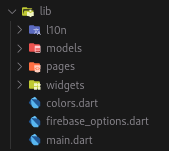
\includegraphics[width=0.35\textwidth]{images/implementacao/frontend/organizacao_projeto.png}
 \caption{Organização do projeto}
 \label{fig:69}
\end{figure}

\begin{itemize}
 \item \textbf{l10n} - Traduções da aplicação;
 \item \textbf{models} - Modelos de classes como \textit{handlers, helpers, providers}, entre outros;
 \item \textbf{pages} - Páginas da aplicação;
 \item \textbf{widgets} - \textit{Widgets} referentes às páginas;
\end{itemize}
\vspace{50mm}



\subsection{Extensions}
A linguagem de programação \textit{dart}, assim como outras linguagens de programação orientadas a objetos, permite alterar e adicionar métodos aos objetos base da linguagem, para realizar isso são criadas extensões do objeto, neste caso foi criada uma extensão para o objeto \textit{string} para facilmente capitalizar um texto.

\subsection{Handlers}
Os \textit{handlers} são porções de código que permitem a execução de ações perante um evento, como por exemplo, realizar uma ação perante um clique no ecrã. Neste caso os \textit{handlers} foram utilizados para detetar o estado da aplicação e realizar ações perante estes estados. Os estados da aplicação referem-se a se a aplicação se encontra em primeiro plano, segundo plano, a resumir ou então desligada. Com estes \textit{handlers} é possível alterar o funcionamento da aplicação perante estes estados, como por exemplo, tratar de notificações da aplicação.

\subsection{Providers}
Os \textit{providers} são classes criadas para ajudar com comunicações externas, neste caso chamadas à \textit{API}, estes foram criados conforme os diversos modelos de dados que se recebem, como por exemplo, uma publicação do fórum. Um \textit{provider} oferece perante um modelo, um conjunto de métodos para as diferentes chamadas necessárias à \textit{API}, como o exemplo anterior, para uma publicação existem métodos para eliminar, adicionar, editar e obter dados, sendo que cada método terá os seus requisitos do serviço que invoca.

Estes \textit{providers} automaticamente detetam a linguagem da aplicação e realizam o pedido ao serviço utilizando essa linguagem.

\subsection{Helpers}
Os \textit{helpers} como o próprio nome indica são classes que ajudam com a realização de tarefas. Neste caso os \textit{helpers}, foram utilizados no auxílio de mensagens de notificações, estas mensagens deveriam conter o nome do utilizador e também a ação do mesmo, traduzida na linguagem da aplicação, pelo que foi criada a classe de \textit{helper} de notificação que contém um método estático para obter a mensagem de uma notificação segundo a ação da mesma.

\newpage

\subsection{Gestão de utilizadores}
Um dos requisitos da aplicação é que apenas as empresas têm a possibilidade de registar-se, pelo que, apenas estas poderão registar os seus técnicos. Dado este requisito foi elaborada a página de gestão de utilizadores, apenas acessível às empresas. Nesta página poderão pesquisar pelos seus técnicos ou registar novos técnicos, sendo que, têm a obrigatoriedade de indicar o nome, \textit{email} e o tipo de técnico. Outras ações que as empresas poderão realizar, é a visualização do perfil de um técnico com a possibilidade de bloquear o acesso ou até apagar a conta do mesmo, sendo que, esta ação é irreversível.

\begin{figure}[htb]%
 \centering
 \subfloat[\centering Aviso de impedir acesso à conta]{{
\includegraphics[width=0.4\textwidth]{images/implementacao/frontend/gestao_users/1686054310970.jpg} }}%
 \qquad
 \subfloat[\centering Aviso de remover conta]{{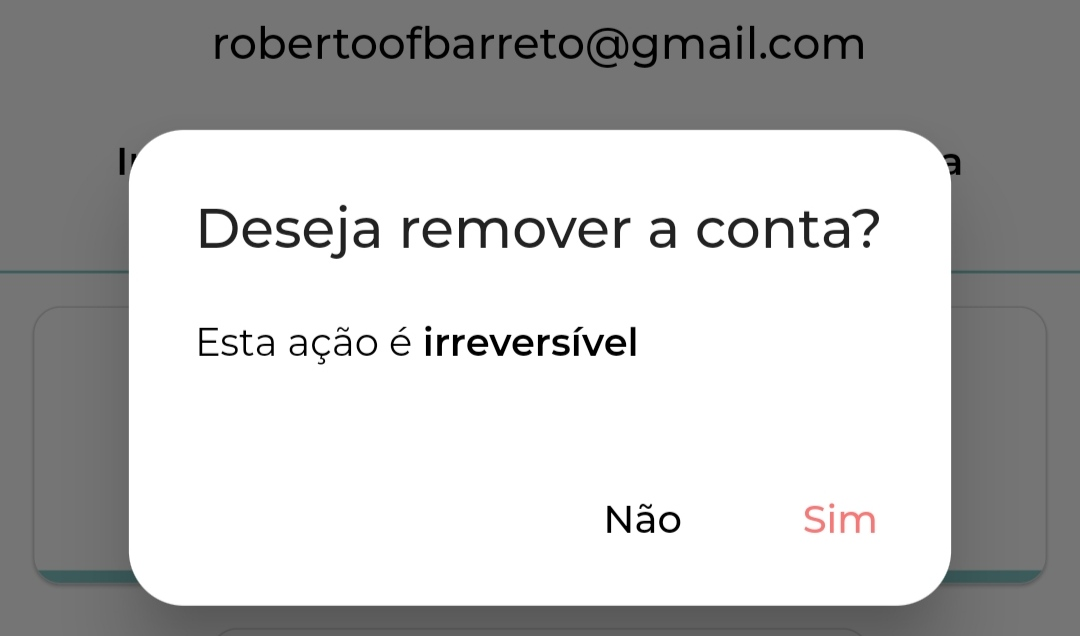
\includegraphics[width=0.4\textwidth]{images/implementacao/frontend/gestao_users/1686054218255.jpg} }}%
 \label{fig:70}%
\end{figure}

Sempre que um utilizador sem acesso ou com a conta apagada efetua o \textit{login}, receberá uma mensagem de erro que menciona que não possui acesso à conta impedindo a continuação do processo.

\begin{figure}[htb]
 \centering
 
\includegraphics[width=0.4\textwidth]{images/implementacao/frontend/gestao_users/1686054218243.jpg}
 \caption{Aviso de login a conta sem acesso}
 \label{fig:71}
\end{figure}

\newpage

\subsection{Fórum}
O desenvolvimento da página do fórum trouxe diversas dificuldades, entre elas, a gestão de filtros, pesquisas, a mostragem de tópicos e atualização dos mesmos.

\vspace{10mm}
\begin{figure}[htb]%
 \centering
 \subfloat[\centering Página de forum]{{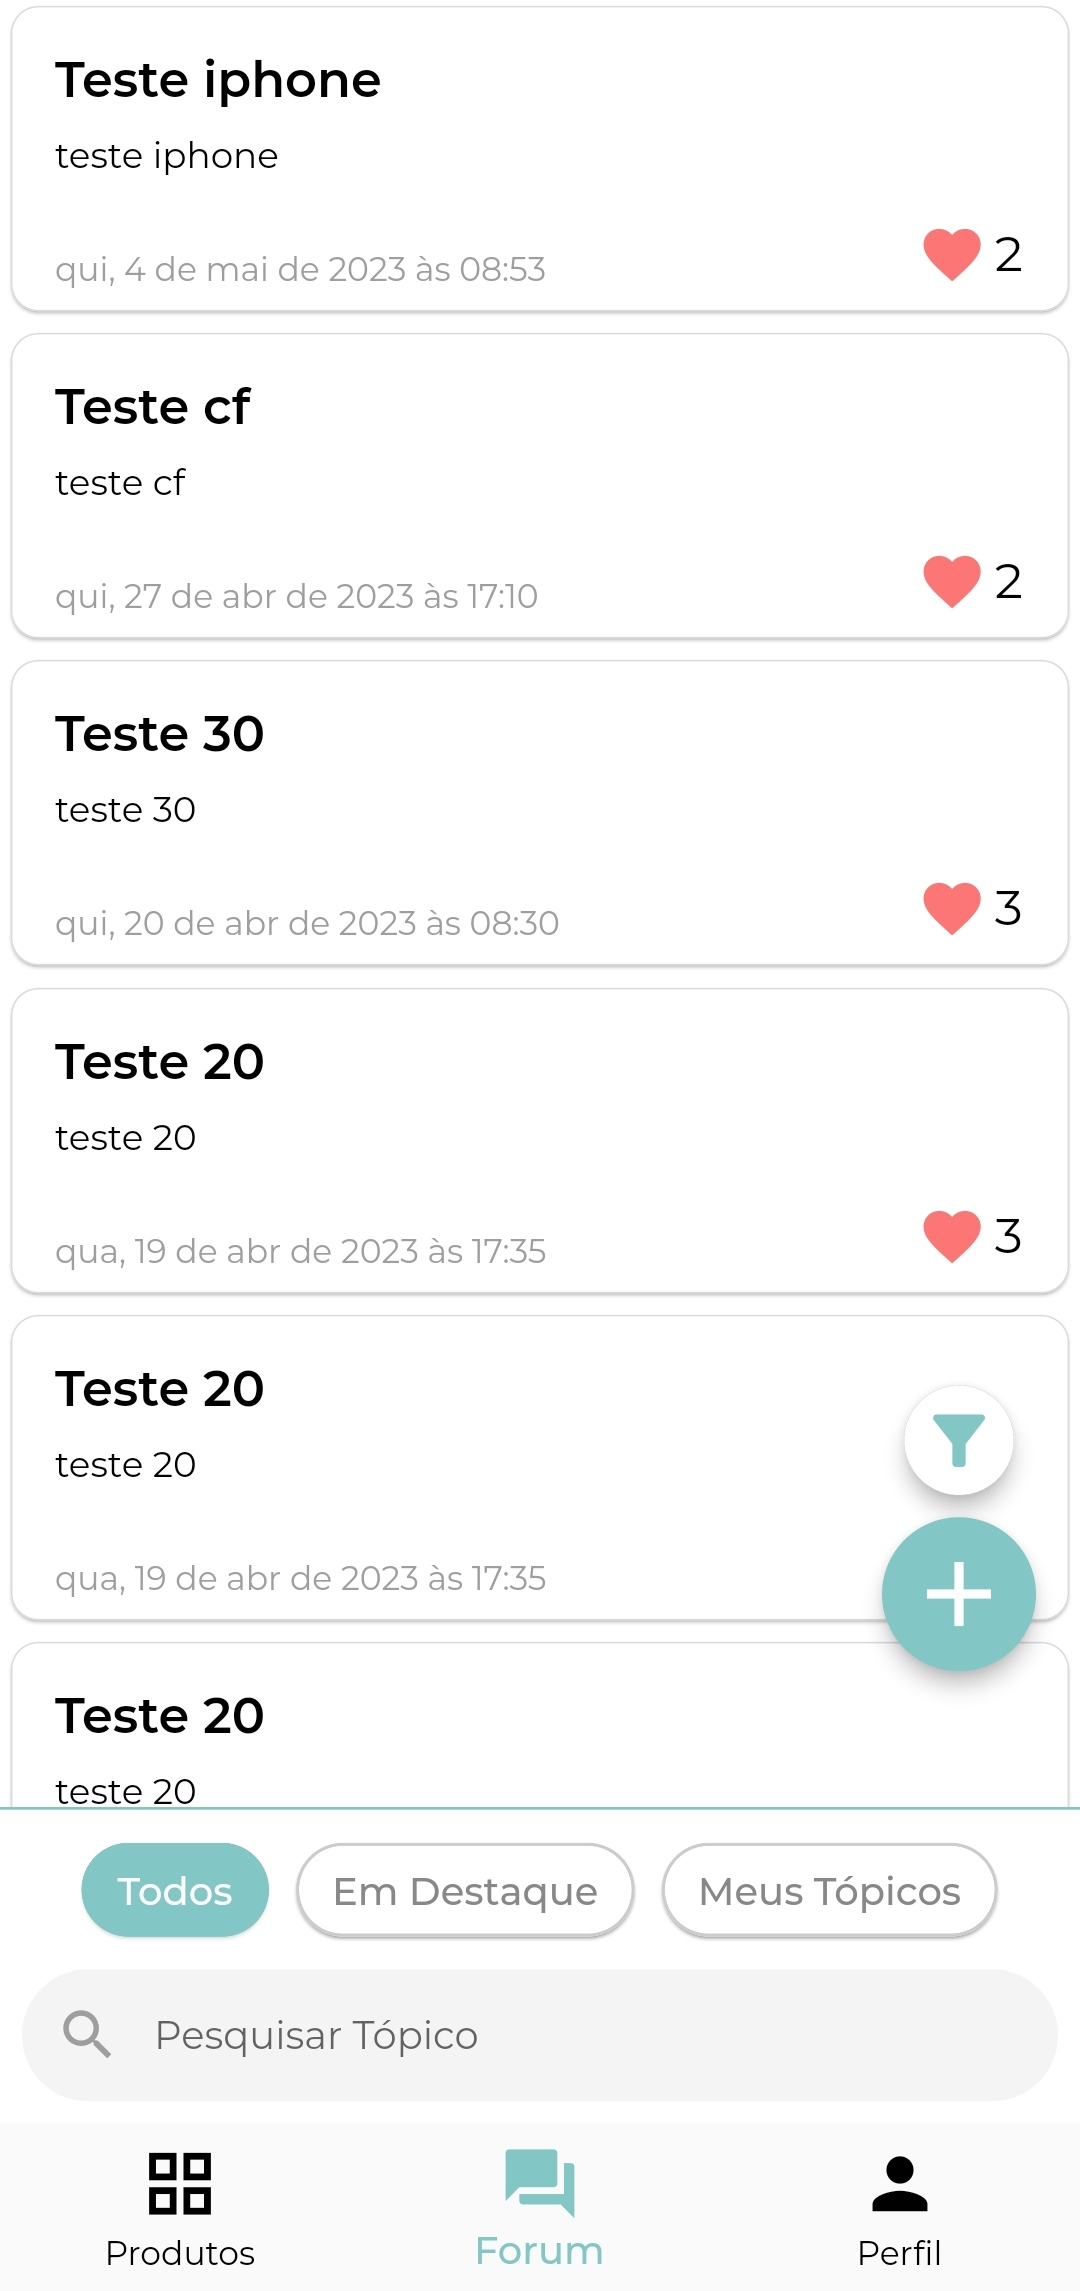
\includegraphics[width=0.4\textwidth]{images/implementacao/frontend/forum/1686055611203.jpg} }}%
 \qquad
 \subfloat[\centering Filtragem de tipo]{{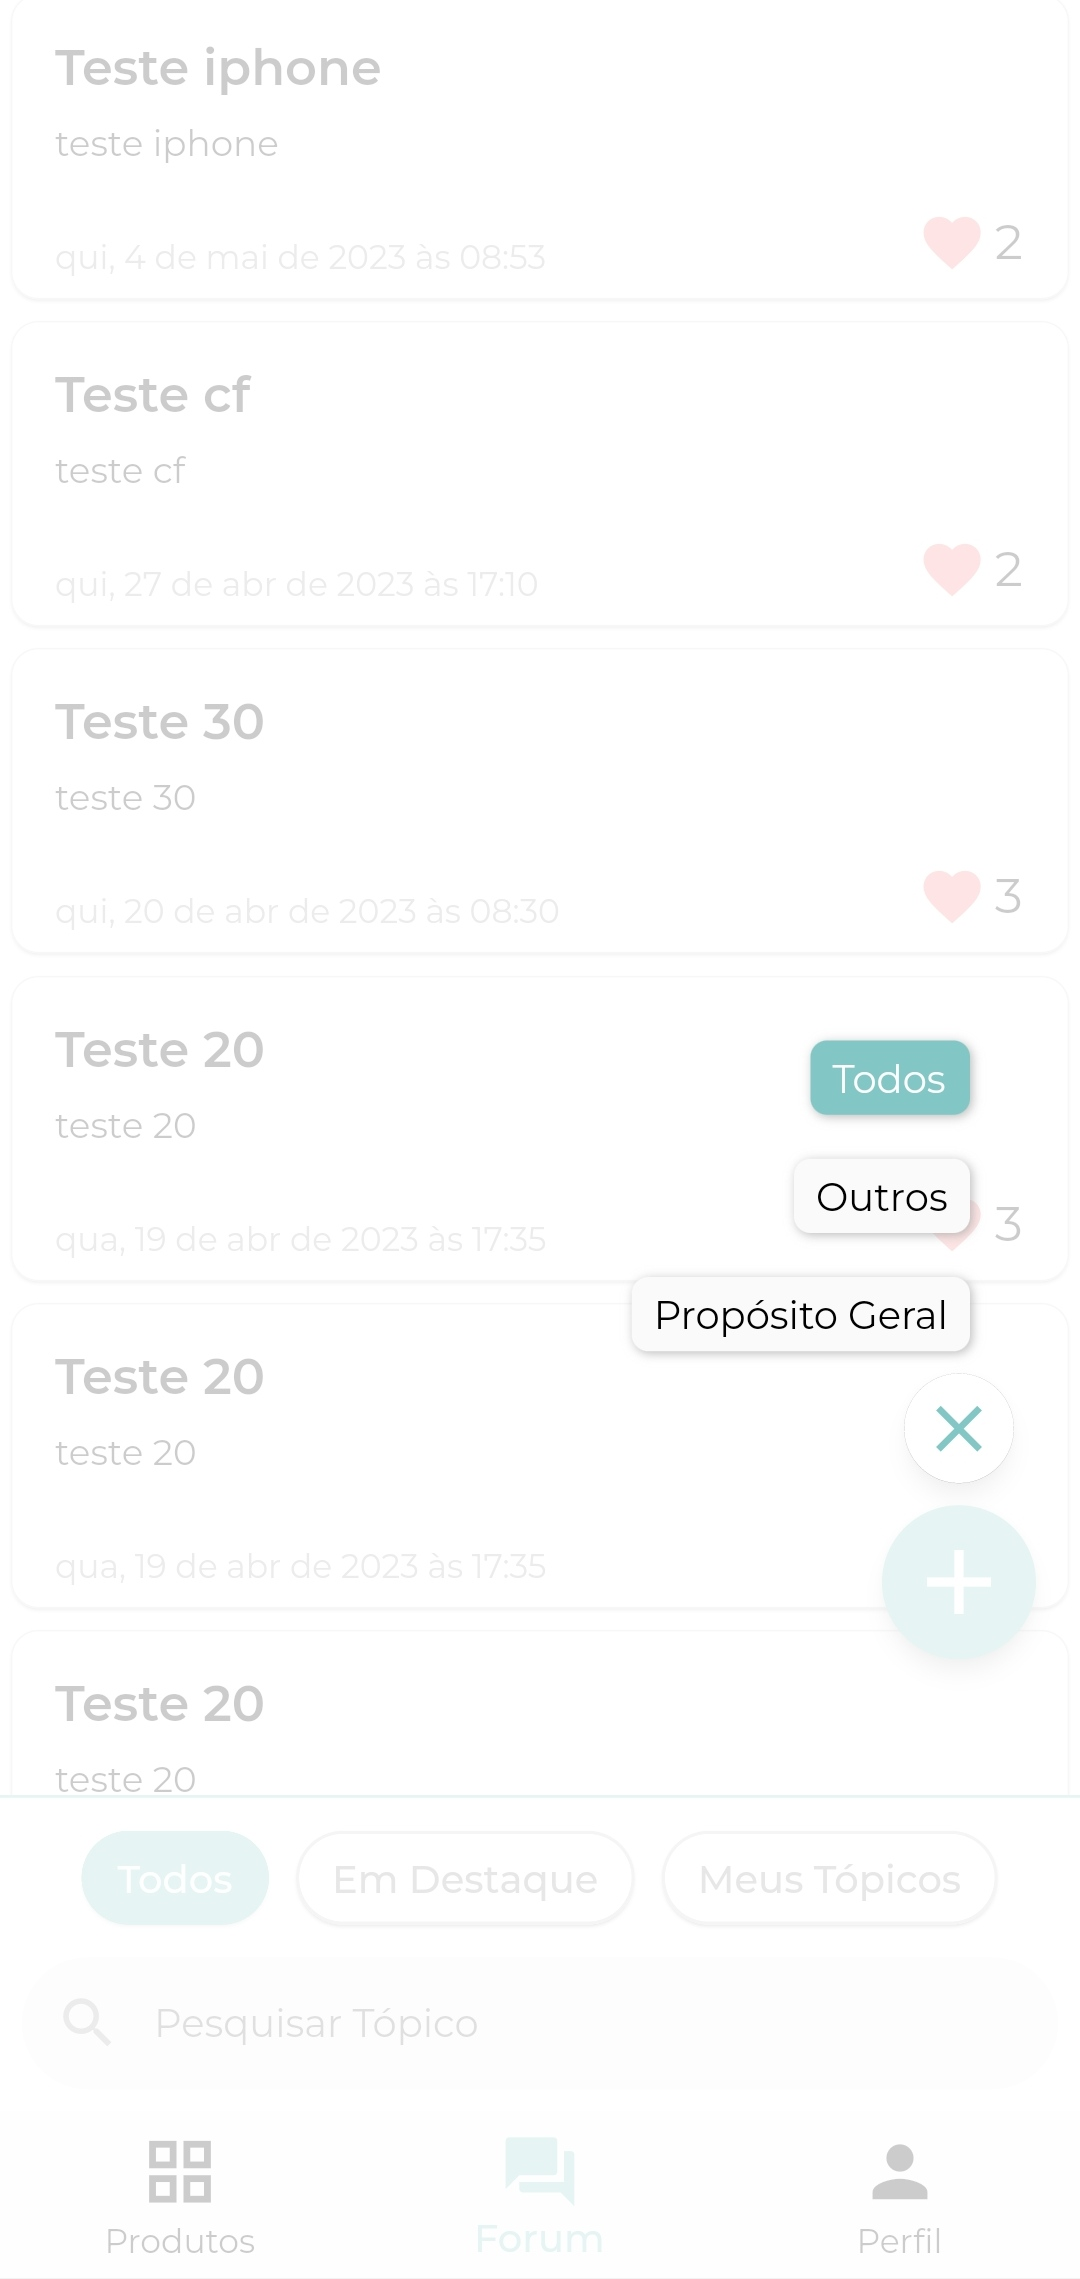
\includegraphics[width=0.4\textwidth]{images/implementacao/frontend/forum/1686055611213.jpg} }}%
 \label{fig:72}%
\end{figure}

\subsubsection{Filtragem de tópicos}
O grande problema com a filtragem dos tópicos é que existem 3 tipos de filtros, o de categoria de tópico, o de tipo de tópico e o de pesquisa. 

Se algum filtro for alterado, os seguintes deverão ser novamente executados para garantir que todos permanecem aplicados. Inicialmente, este tipo de filtragem não era realizado, o que levava a diversos problemas, tais como, na realização de uma pesquisa, esta não era efetuada sobre os tópicos filtradas, o que levava a que a pesquisa fosse efetuada por todos os tópicos.

Outro problema detetado foi a troca de categorias, que por vezes, os filtros adicionavam-se, o que levava a que estes não apresentassem tópicos.

Sendo assim, foram criados métodos para auxílio na filtragem, tais como, uma prioridade, onde cada método invoca o método seguinte de forma encadeada. Primeiramente aplica-se o filtro de categoria, de seguida este envia o resultado para o método de filtragem por tipo e por fim, se existir algum tipo de pesquisa, os tópicos provenientes do método anterior serão filtrados.

\begin{figure}[htb]
 \centering
 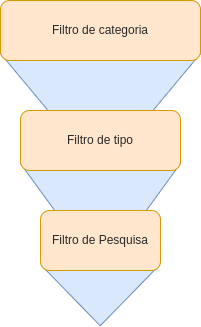
\includegraphics[width=0.3\textwidth]{images/implementacao/frontend/forum/filtros/filtros.png}
 \caption{Filtragem do forum}
 \label{fig:73}
\end{figure}

\subsubsection{Carregamento de tópicos}
Inicialmente o carregamento de tópicos fazia-se por inteiro, desde carregamento de todos os tópicos, até todos os dados dos mesmos, visto que, não existiam muitos tópicos este não seria um problema para a \textit{\acrshort{api}}, mas, conforme os testes foram realizados a quantidade de tópicos existentes foi gradualmente aumentando, pelo que, foi possível visualizar o tempo de demora da resposta do servidor a aumentar, assim como, o desempenho da aplicação no fórum a piorar.

A resolução deste problema proveio com uma técnica de \textit{sliding window}, na qual os tópicos mantêm-se carregados, sendo que, a própria \textit{framework} consegue através da lista retirar de renderização os tópicos que o utilizador não consegue ver. 

Esta solução foi implementada através da utilização de três valores, quantidade de tópicos a obter, índice inicial e data do primeiro tópico. O valor de quantidade de tópicos a obter, inicialmente dez, permite limitar a quantidade de tópicos que a \textit{\acrshort{api}} irá processar, o que reduz o tempo de resposta. O índice inicial, indica qual o índice do primeiro elemento que se deseja obter da lista. A data do primeiro tópico, mantém uma referência temporal para obter tópicos, o que garante que a lista que está ser a visualizada é sempre a mesma.

Também foi reduzida a quantidade de dados carregados por cada tópico, pelo que, apenas os comentários diretos ao tópico são carregados e não as respostas a estes, o que contribuiu para a melhoria do desempenho.

\newpage

Por fim, sempre que o utilizador alcança o fim da lista de tópicos este poderá deslizar para carregar mais tópicos.

Encontra-se no documento de anexos, no anexo 27, uma versão mais detalhada da Figura~\ref*{fig:74}.

\begin{figure}[htb]
 \centering
 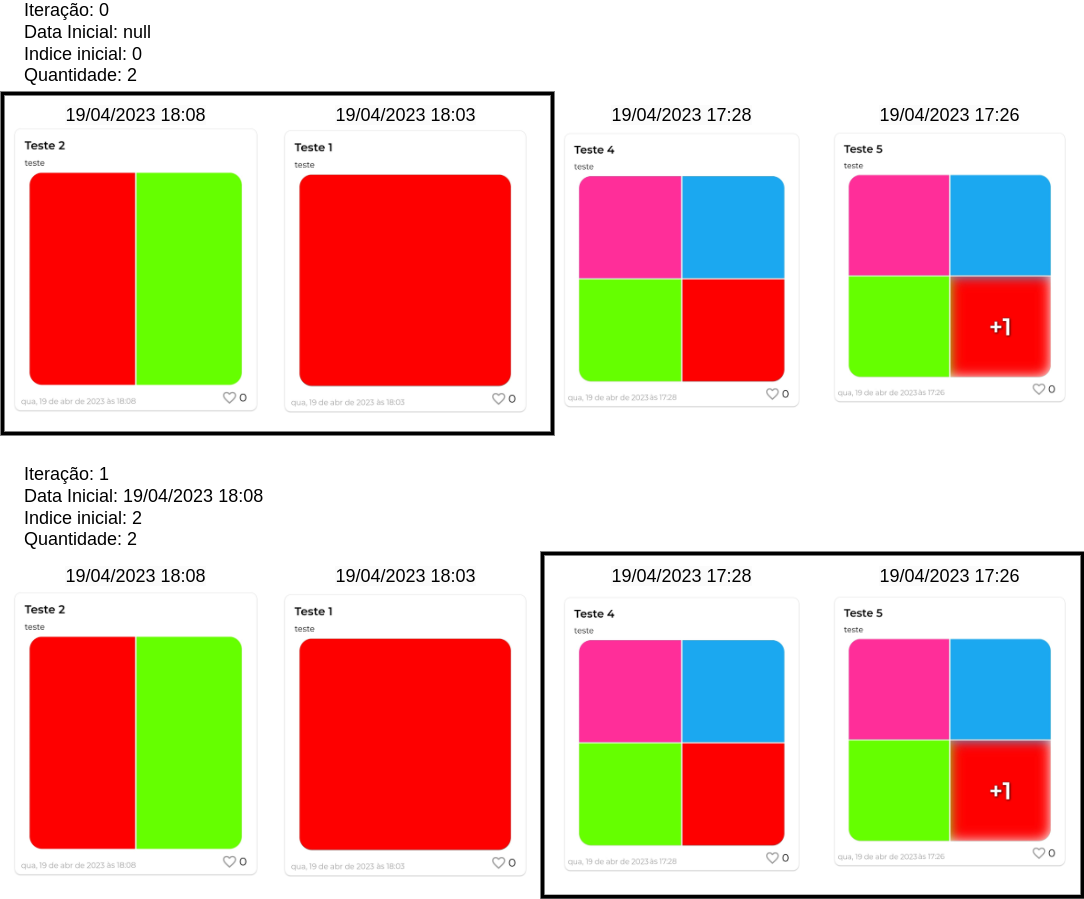
\includegraphics[width=0.85\textwidth]{images/implementacao/frontend/forum/loading_topics/topics_loading.png}
 \caption{Carregamento de tópicos}
 \label{fig:74}
\end{figure}

\subsubsection{Detalhes de tópico}

A página de detalhes de tópico sofreu os mesmos problemas que a página anterior, o que levou à necessidade de aplicar a mesma solução sobre os comentários de tópico e sobre as respostas aos mesmos. Sendo assim são carregados os primeiros dez comentários e por fim, demonstrado ao utilizador quantos mais existem que poderá carregar, sendo carregados dez de cada vez.

Estes comentários podem conter respostas, sendo que estas conseguem ser carregadas também dez de cada vez e o utilizador consegue esconder ou mostrar estas.

Outro problema que surgiu no desenvolvimento da página de detalhes de tópico foi o destaque de um comentário. Este foi uma grande dificuldade, pois, com a nova implementação as mensagens não estão carregadas no momento do destaque da mensagem, pelo que, é necessário procurar a mesma nos comentários carregados, o que expande as respostas do comentário que contêm a reposta a destacar.

\newpage

O destacamento das mensagens também continha um erro. Sempre que algo no ecrã é atualizado, este recarregava a animação de destaque, como solução este código foi movido para apenas ser executado no momento de inicialização do ecrã após todos os elementos se encontrarem devidamente carregados.

\begin{figure}[htb]
 \centering
 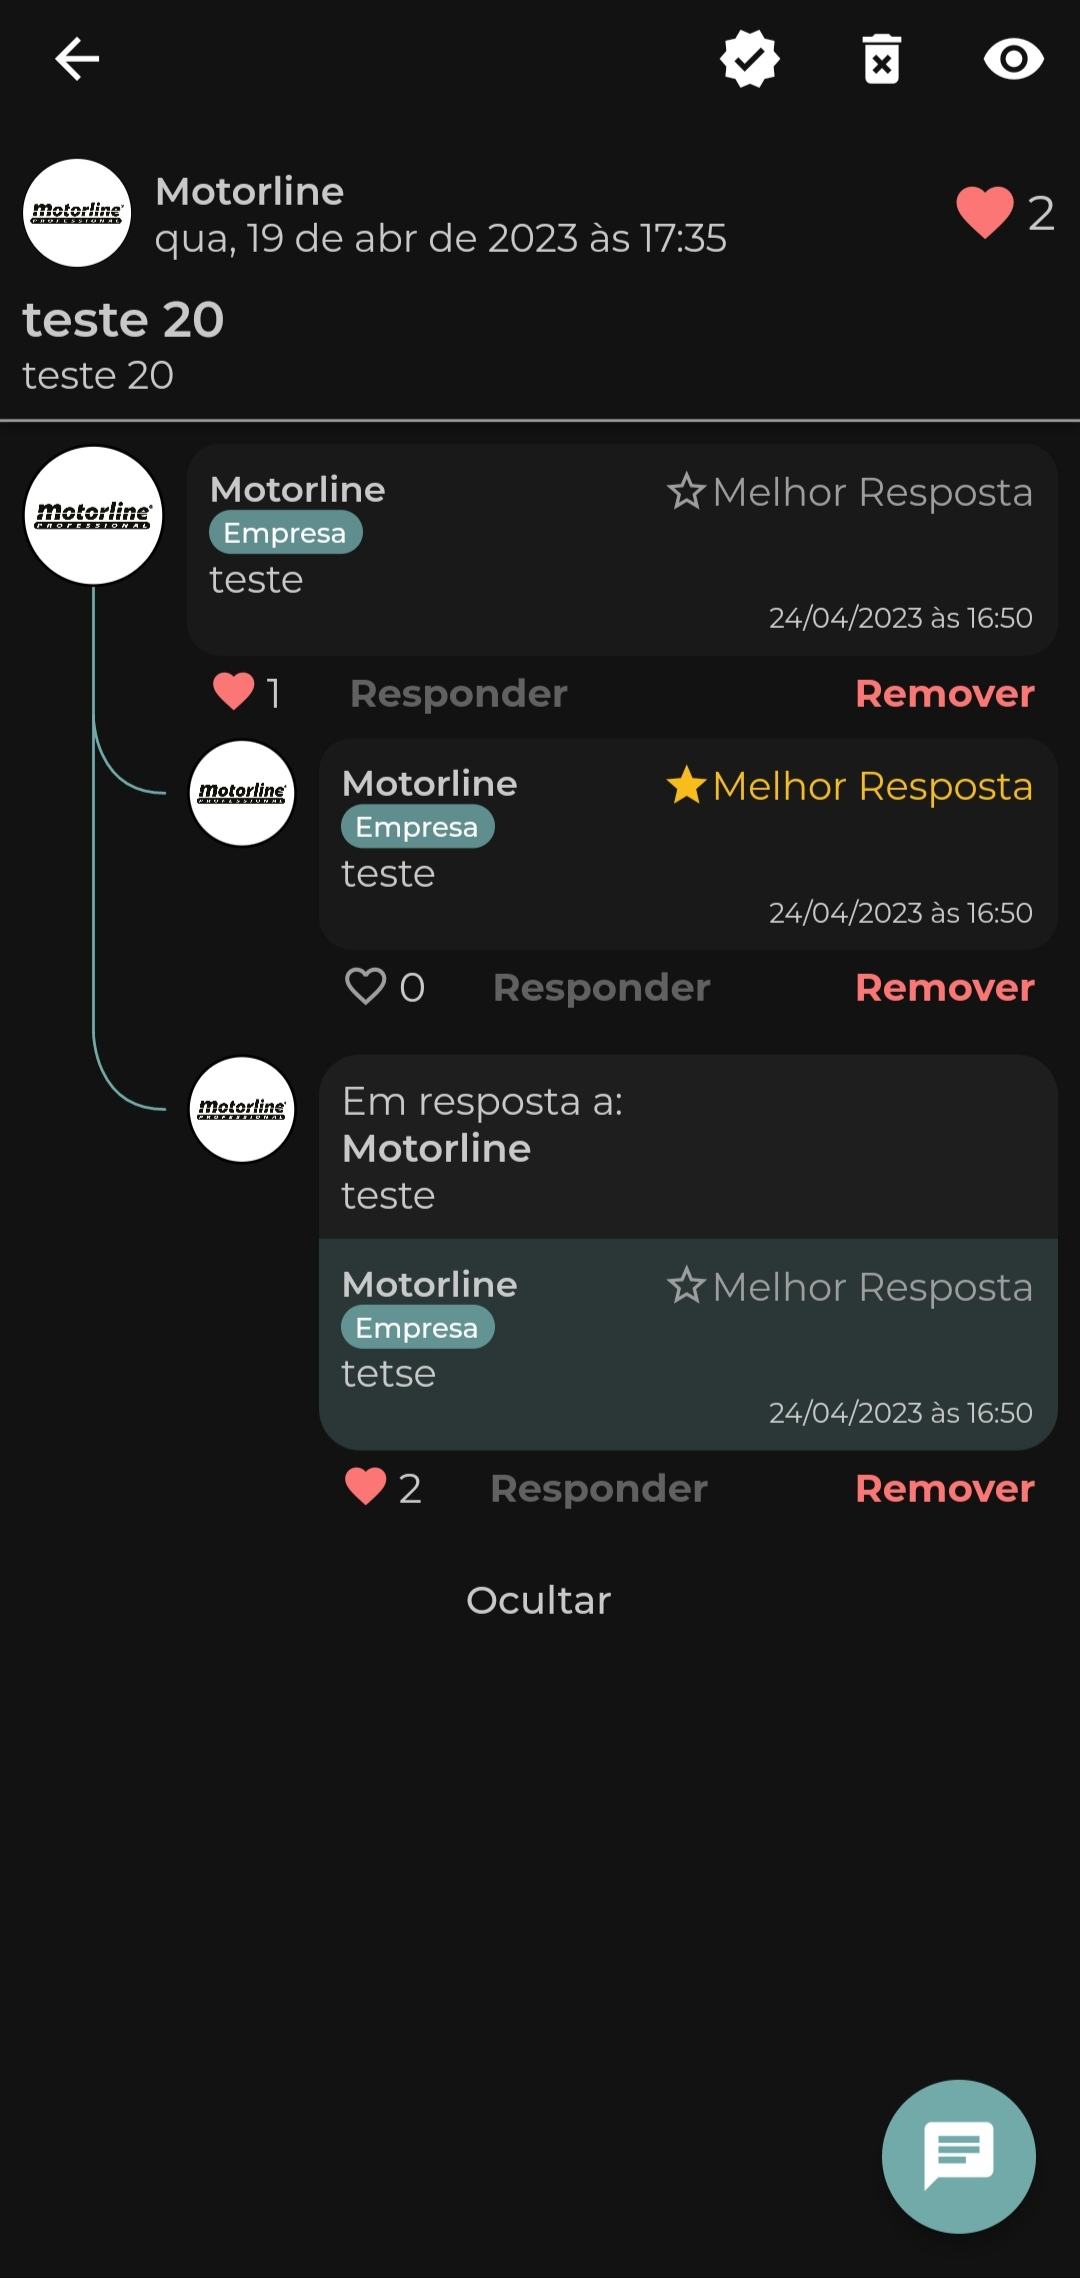
\includegraphics[width=0.35\textwidth]{images/implementacao/frontend/forum/loading_topics/1686062701127.jpg}
 \caption{Destaque de mensagens}
 \label{fig:75}
\end{figure}

\subsection{Firestorage}

Visto que a desenvolvedora do \textit{Flutter} e do \textit{Firebase} é a mesma, esta disponibilizou recursos que facilitam a utilização desta ferramenta pelo \textit{Flutter}, sendo assim todas as imagens e vídeos de utilizadores, publicações e comentários são guardadas diretamente da aplicação para o \textit{firestorage}, assim como o acesso às mesmas é realizado diretamente.

Para permitir este tipo de acesso o \textit{Firebase} disponibiliza de uma ferramenta que permite através do terminal configurar a ligação entre o projeto e o servidor do \textit{Firebase}, sendo que no final apenas é necessário importar a biblioteca do serviço do \textit{Firebase} que se deseja e invocar a classe do mesmo para realizar alguma ação.

Os ficheiros são então organizados conforme o seu contexto. Para utilizadores existe a pasta utilizadores, para tópicos existe a pasto tópicos e para comentários existe a pasta comentários. 


A pasta utilizadores, como cada utilizador, apenas contém uma imagem, então estas são guardas com o nome do id do utilizador e na eventualidade de já existir é substituída. No caso de tópicos e comentários como podem conter várias imagens e vídeos, então estes são guardados em pastas com os ficheiros referentes e que têm por nome os ids dos tópicos ou comentários.

\begin{figure}[htb]%
  \centering
  \subfloat[\centering Raiz do firestorage]{{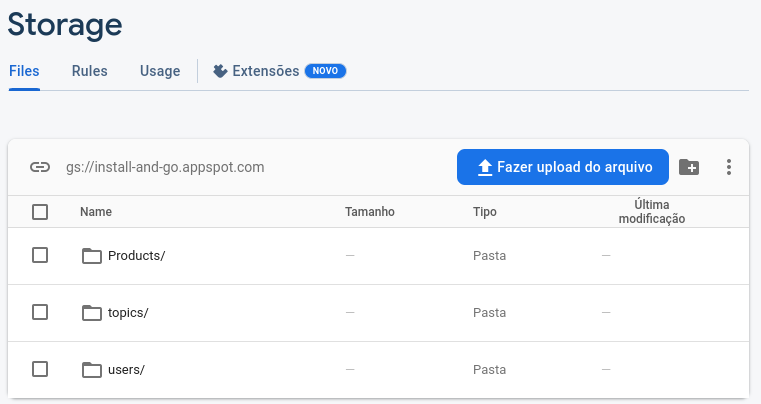
\includegraphics[width=0.7\textwidth]{images/implementacao/frontend/firestorage/all.png} }}%
  \qquad
  \subfloat[\centering Pasta topics do firestorage]{{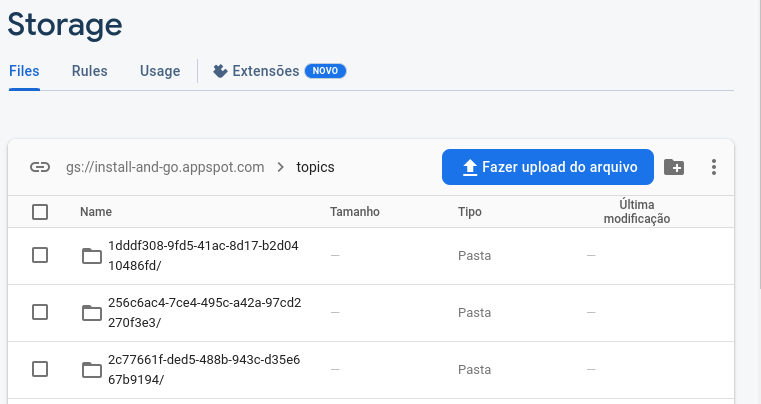
\includegraphics[width=0.7\textwidth]{images/implementacao/frontend/firestorage/topics.png} }}%
  \label{fig:76}%
\end{figure}

\subsection{Apresentação de Imagens}
A apresentação de imagens é definida em 2 niveis, a nivel de pré-visualização, por exemplo ver a miniatura da imagem de uma publicação no forum e a nivel de detalhe, onde é possivel ver a imagem em ponto grande e realizar zoom na mesma.

Para a apresentação de miniatura da imagem foi decidido mostrar até 4 imagens, sendo que acima de 4 imagens seria mostrado apenas 3 imagens significando assim que a quarta imagem indicaria quantas mais imagens existem para mostrar. 

Para a implementação da apresentação das miniaturas de imagens, foi utilizada a biblioteca staggered\_grid\_view, esta biblioteca permite organizar imagens em grelha. Neste contexto desejava-se organizar estas imagens em diferentes aspetos, e disposições, pelo que esta biblioteca permite indicar quantas colunas e linhas existem na grelha ao criar o agrupamento de imagens, sendo assim foi decidido que quando são duas imagens estas dividem a grelha, quando são três imagens a primeira divide metade da grelha e as outras duas dividem a outra metade, quando são 4 ou mais então as 4 imagens dividem a grelha por igual. Quando se encontram existentes mais do que 4 imagens foi então decidido colocar um filtro de desfoque sobre a ultima imagem e colocar por cima desta quantas mais imagens existem para mostrar.

\begin{figure}[htb]%
  \centering
  \subfloat[\centering Publicação com 5 imagens]{{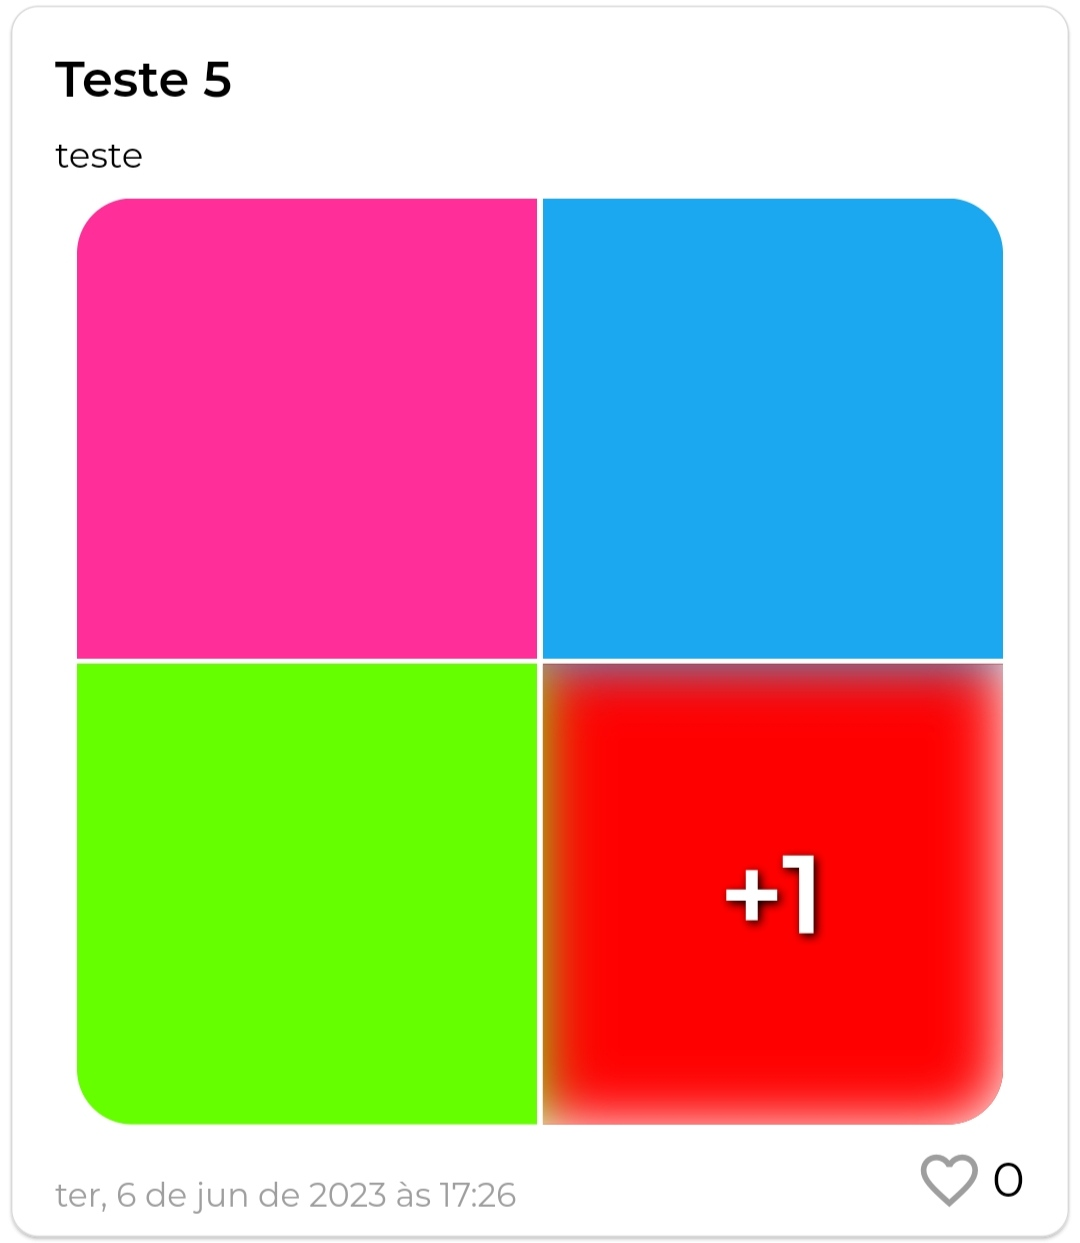
\includegraphics[width=0.2\textwidth]{images/implementacao/frontend/apresentacao_imagens/1686068843028.jpg} }}%
  \qquad
  \subfloat[\centering Publicação com 4 imagens]{{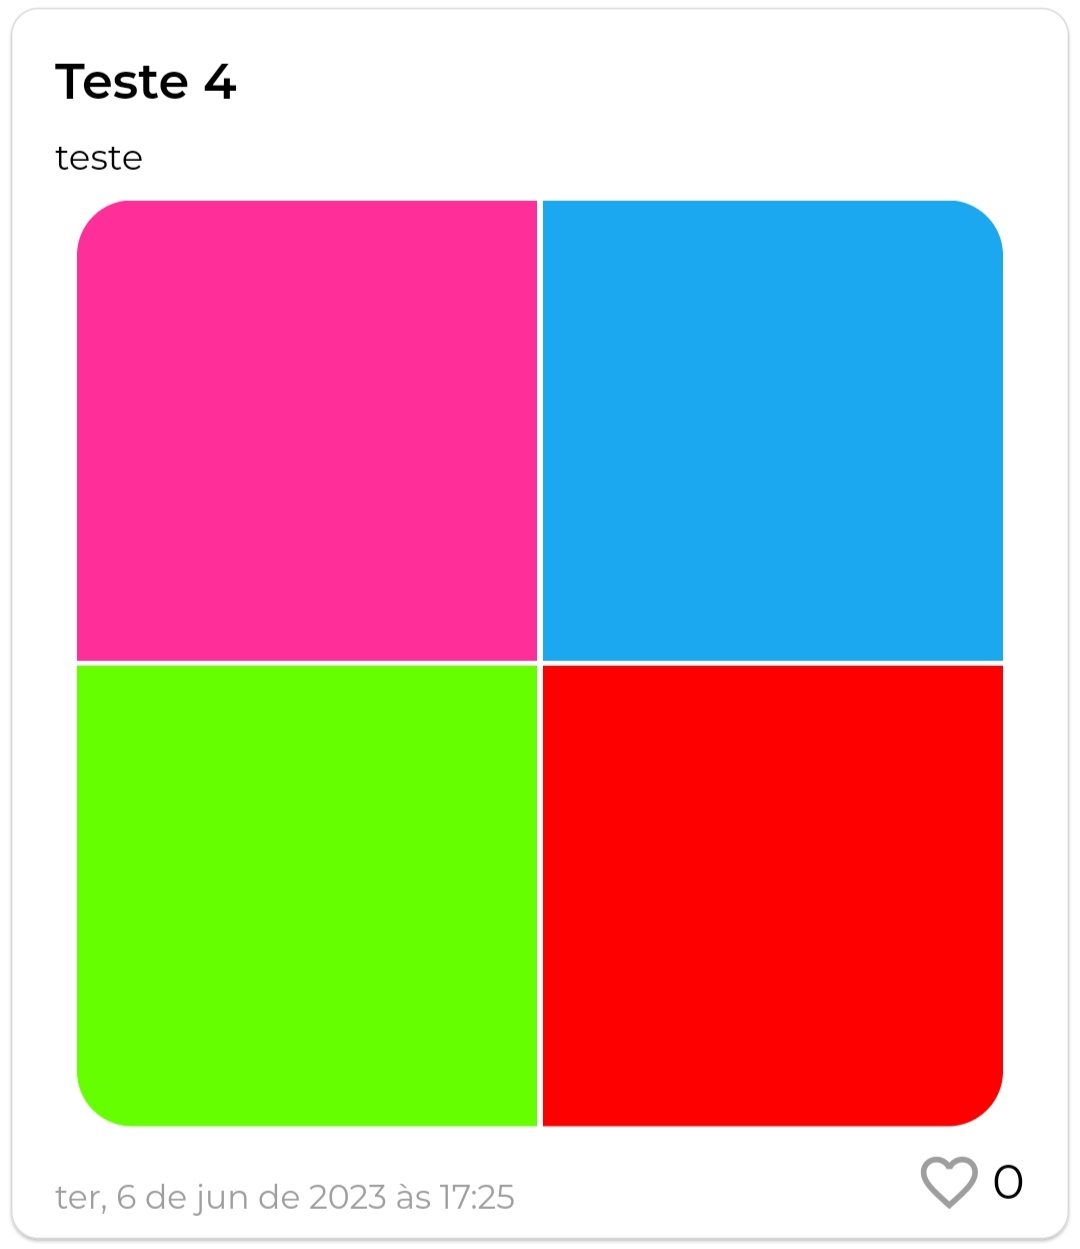
\includegraphics[width=0.2\textwidth]{images/implementacao/frontend/apresentacao_imagens/1686068843039.jpg} }}%
  \qquad
  \subfloat[\centering Publicação com 3 imagens]{{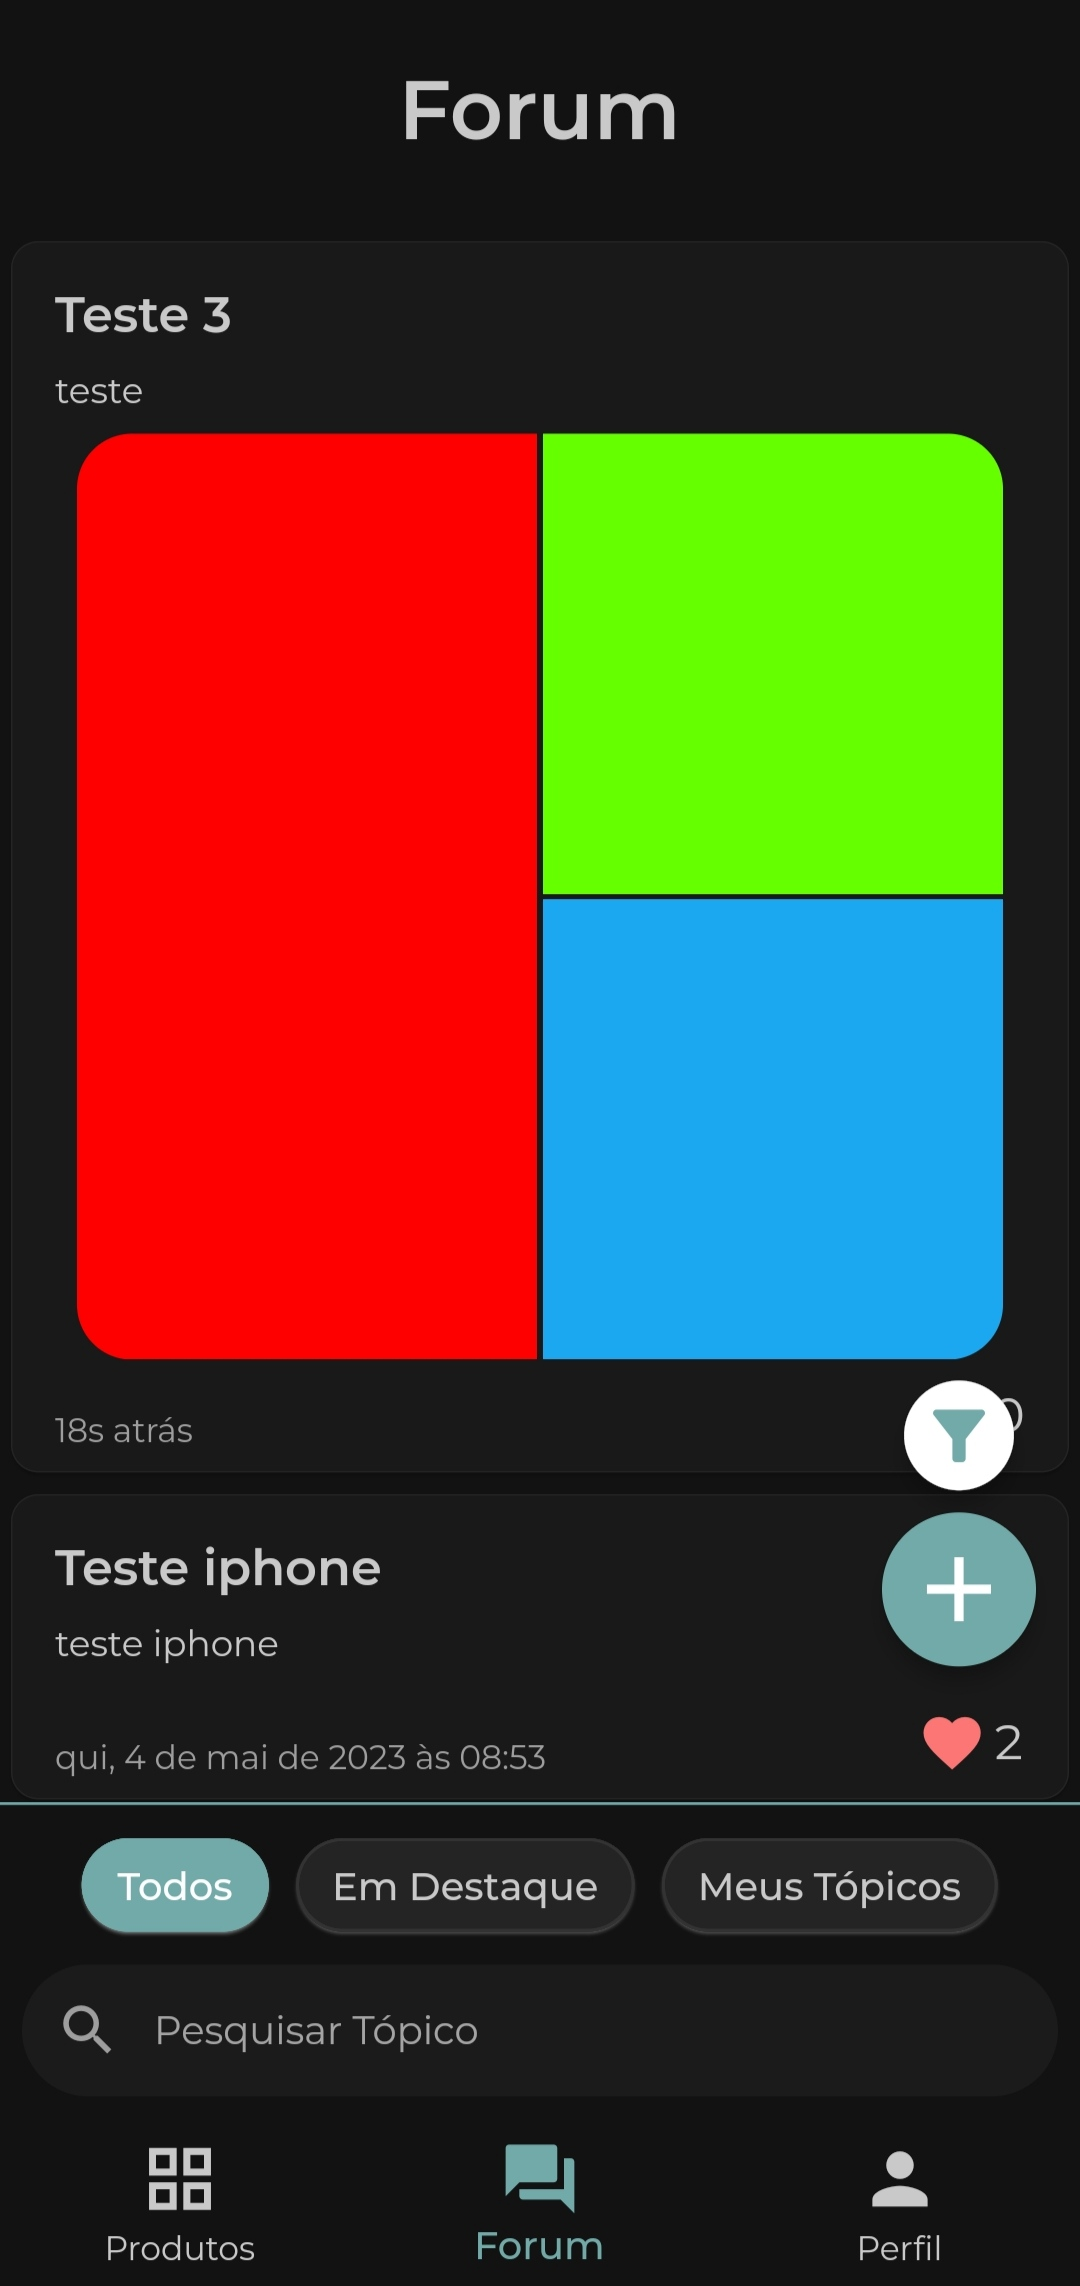
\includegraphics[width=0.2\textwidth]{images/implementacao/frontend/apresentacao_imagens/1686068843051.jpg} }}%
  \label{fig:76}%
\end{figure}

\subsection{Apresentação de Imagens em carrosel}

A apresentação de imagens deverá permitir que o utilizador as visualize em ponto grande conseguindo também realizar diversas ações sobre estas, para isso foram experimentadas diversas bibliotecas, mas nunca se conseguia o comportamento desejado, sendo assim foi decidido criar o próprio carrosel de imagens, sendo que o próprio flutter já disponibiliza um widget para tal.

O ponto de maior dificuldade para este processo foi a implementação de zoom, visto que o flutter não dispõe de widgets para tal, sendo assim foi necessário primeiramente detetar gestos com o detetor de gestos da ferramenta e aplicado um zoom sobre o centro do gesto, os gestos aceites foram o de pinça e o gesto de duplo clique.

O grande problema com esta solução é que visto que é permitido um scroll horizontal de imagens os gestos por vezes poderão não funcionar corretamente, principalmente o gesto de pinça que se efetuado na horizontal poderá resultar em scroll horizontal. Para resolver tal problema foi decidido que quando dois dedos são detetados no ecrã a navegação horizontal fica bloqueada e assim que estes são levantados, a navegação horizontal é ativada novamente.

\newpage

\subsection{Carregamento de Imagens}

O carregamento de imagens do dispositivo poderá ser realizado por meio de seleção de imagens da galeria, para realizar este tipo de seleção primeiramente foi testada a biblioteca image\_picker, mas esta biblioteca utiliza o seletor de ficheiro do dispositivo, o problema é que este tipo de seleção permite também a seleção de ficheiros também o que faz com que seja necessário um conjunto de outras verificações para garantir que apenas as imagens são selecionadas o que levaria a uma possível perda de performance e perda de qualidade na experiencia de utilização do utilizador.

Sendo assim foi de seguida testada a biblioteca advance\_image\_picker, mas o problema desta biblioteca é que não permite selecionar vídeos, pelo que foi decidido experimentar a biblioteca wechat\_asset\_picker, esta biblioteca cria uma página de seleção de imagens própria para seleção de imagens e vídeos diretamente da galeria, esta permite indicar o limite máximo de seleção e os tipos de ficheiros que o utilizador poderá selecionar de forma a que apenas os tipos aceites são mostrados, acrescentando também que esta biblioteca permite visualizar a tipagem de cada ficheiro no próprio objeto, o único ponto desvantajoso é que não é possível traduzir o botão de confirmação de seleção.

Após a carregar os ficheiros para memória, estes são então enviados para o firestorage como mencionado anteriormente.

\newpage

\subsection{Vídeos}

A maior dificuldade detetada nos vídeos foi a necessidade de um comportamento diferente nestes quando se encontram no ecrã de visualização de imagens e vídeos, visto que, ao contrário das imagens, os vídeos necessitam de um \textit{player}, sendo sempre necessário verificar qual o tipo de ficheiro antes de carregar o \textit{widget} do mesmo.

Para resolver o problema de utilizar um \textit{player} testou-se uma biblioteca que permite a utilização do \textit{player} nativo do dispositivo, ou seja, \textit{android} utilizaria o \textit{player} do \textit{android} e \textit{ios} utilizaria o \textit{player} de \textit{ios}. O grande problema com esta solução é que o \textit{player} de \textit{android} tem os botões completamente brancos, sem nenhum tipo de fundo para os destacar, o que significa que se um vídeo branco for visualizado, o utilizador não conseguirá visualizar os botões do \textit{player}.

Deste modo decidiu-se desenvolver um \textit{player} próprio. Após a implementação de diversas funções como, pausar, resumir, avançar 5 segundos e recuar 5 segundos, esconder e apresentar os botões, existiam dois grandes problemas, demonstrar o vídeo em ponto grande, voltar para o mesmo tempo do vídeo em ponto pequeno e também o comportamento do \textit{player} não ser completamente fluido.

Depois de uma vasta pesquisa compreendeu-se que o \textit{player} do \textit{ios} resolvia os problemas do \textit{player} do \textit{android} através da colocação de um fundo nos botões do \textit{player}. Através da biblioteca \textit{appinio} é possível utilizar e configurar o \textit{player} nativo de \textit{ios} em \textit{android}. Sendo assim, a utilização do \textit{player} de \textit{ios} em ambos os sistemas operativos resolveria o problema. Este \textit{player} permitiu a resolução de um problema menor, a visualização de vídeos em ponto grande, sendo que, dependendo da orientação do vídeo, o \textit{player} altera a orientação da aplicação automáticamente voltando à orientação vertical, uma vez que, termina a visualização do vídeo em ponto grande.

\subsection{Links}
Uma das funcionalidades necessárias da aplicação é a utilização de \textit{links}. Para isto, a programação \textit{mobile} oferece duas soluções, \textit{app links}, \textit{deep links} e \textit{dynamic links}. Como mencionado na secção de tecnologias foi decidido implementar a solução de \textit{dynamic links} da \textit{Firebase}.

Para implementar esta solução, primeiramente a nível de \textit{backend} foi necessário gerar os \textit{links}, para isto, existem duas opções, implementação do \textit{Firebase} no próprio \textit{backend} ou então uma chamada ao \textit{Firebase} com a utilização de uma chave de pedido. Em primeiro lugar foi testada a implementação do \textit{Firebase} no próprio \textit{backend}, contudo, esta implementação surgiu com alguns problemas, uma vez que, existem diversas configurações específicas necessárias, sendo então recomendado pelos colegas de trabalho a chamada ao \textit{Firebase} dada à sua simplicidade.

Sendo assim, para a realização de chamadas ao \textit{Firebase} foi utilizado o \textit{axios}. Este permitiu realizar um pedido com o método \textit{POST} para o serviço de \textit{dynamic links} do \textit{Firebase}, com indicação do prefixo do projeto. Para permitir a reutilização deste código foi colocado num método onde é chamado com indicação do \textit{link} desejado e os dados a enviar. O \textit{link} é utilizado para, por exemplo, como numa página \textit{web}, indicar qual página se deseja direcionar o utilizador, já os parâmetros, assim como em um \textit{url web}, são enviados através do próprio \textit{link}, pelo que, estes dados são colocados na \textit{string} do \textit{link} o que permite a configuração perante diversas situações. Por fim, a \textit{Firebase} retorna o \textit{link} criado e este é colocado no \textit{email} desejado.

Para a implementação do \textit{frontend} foi necessário importar a biblioteca de \textit{dynamic links} do \textit{Firebase} e de seguida no código de inicialização da aplicação colocar um método para em caso de a aplicação ser aberta a partir de um \textit{link}, este o ler. Quando este método lê o \textit{link}, extrai a página indicada e a lista de parâmetros recebidos. Deste modo, o utilizador é redirecionado para a página do \textit{link} com os dados recebidos.

Aquando o teste da implementação, diversas tentativas de abertura de \textit{links} foram realizadas, mas, contudo, sem sucesso. A grande dificuldade desta implementação foi os \textit{links} dinâmicos não permitem realizar \textit{debug}, sendo que, ou funcionará na totalidade, ou não funcionará, o que leva a que seja complicado identificar \textit{bugs}. A documentação do serviço foi de grande auxílio, uma vez que, estava em falta a indicação do nome do pacote da aplicação para \textit{Android} e \textit{iOS}. Após a colocação destes dados, tudo seguiu em completo funcionamento.

\subsection{Notificações}

A implementação de notificações revelou-se ser a implementação de maior dificuldade devido a diversos imprevistos da mesma. Para isto foi utilizado o serviço de notificações do \textit{Firebase}, este surge assim como os \textit{links}, em 2 secções, primeiramente \textit{backend} e de seguida \textit{frontend}.

A nível de \textit{backend} foi necessário utilizar \textit{axios} para realizar um pedido ao serviço de notificações do \textit{Firebase}, mas assim como na criação dos \textit{links} o serviço não indica quaisquer informações sobre erros, apenas o dispositivo poderá ou não receber a notificação. 

Em primeiro lugar, foi utilizado o conteúdo a enviar indicado pela documentação do serviço, mas apenas retornava uma mensagem de erro, de seguida foi pesquisado outras implementações de outros utilizadores e testado, mas novamente surgia um erro, pelo que foi decidido utilizar o conteúdo indicado pelo professor de programação de dispositivos móveis, tendo este funcionado sem qualquer indicação de erro. 

No conteúdo da notificação é enviado em formato \textit{json} a mensagem a mostrar na notificação e como estas serão sempre referentes a tópicos ou comentários, então é indicado o \textit{id} do tópico, do comentário e em caso de necessidade o \textit{id} do comentário pai.

Este processo de notificação foi também aproveitado para direcionar os mesmos dados para notificação de \textit{email} em caso do utilizador possuir ativo as notificações por \textit{email}, sendo gerado um \textit{link} dinâmico com os dados na notificação.

A nível de \textit{frontend} foi importada a biblioteca do serviço de notificações do \textit{Firebase}, sendo esta implementada conforme a documentação. Uma vez que é necessário detetar notificações no iniciar da aplicação, durante a utilização e quando esta se encontra em segundo plano, foi aproveitado estas deteções para implementar o direcionamento do utilizador para as páginas referentes às notificações, utilizando os dados recebidos.

O grande problema encontrado com as notificações é que o \textit{icon} não era mostrado corretamente sendo que ou era mostrado um quadrado escuro, ou nenhum \textit{icon}. A biblioteca de notificações do \textit{Firebase} não permite a customicação do \textit{icon} da mesma, pelo que foi decidido utilizar a biblioteca \textit{flutter\_local\_notifications}, esta permite a total customização das notificações sendo então enviado o icon desenhado para a aplicação. Mesmo assim as notificações continuavam com o mesmo erro, pelo que foi decidido realizar uma pesquisa e foi percebido que \textit{android} possui um novo sistema para os \textit{icons} das notificações pelo que é necessário transformar estes em preto ou branco com fundo transparente e de seguida tratados pelo próprio \textit{android}.

Sendo assim foi realizada a transformação e novamente alterados os \textit{icons} das notificações, após uma nova testagem foi percebido que mesmo assim apenas o \textit{icon} da notificação expandida teria sido alterado, após uma nova pesquisa foi percebido que \textit{android} necessita de 2 \textit{icons} de notificação para aplicar a ambas as situações, tendo sido assim resolvido o problema em questão.

Nesta implementação apenas um problema continuou sem resolução, a abertura de notificações quando a aplicação se encontra terminada, foram testadas várias soluções, mas após a leitura de documentação e de soluções de outros utilizadores, foi percebido que o \textit{Flutter} não permite a reconfiguração do comportamento de notificações quando a aplicação se encontra terminada. O \textit{Flutter} possui como futura implementação a permissão de reconfiguração do comportamento do \textit{click} neste tipo de notificação, mas de momento não dispõe de solução.

\input{sections/chap4/3.frontend/10.permissões.tex}

\newpage

\subsection{Ios}